% This is "sig-alternate.tex" V2.0 May 2012
% This file should be compiled with V2.5 of "sig-alternate.cls" May 2012
%
% This example file demonstrates the use of the 'sig-alternate.cls'
% V2.5 LaTeX2e document class file. It is for those submitting
% articles to ACM Conference Proceedings WHO DO NOT WISH TO
% STRICTLY ADHERE TO THE SIGS (PUBS-BOARD-ENDORSED) STYLE.
% The 'sig-alternate.cls' file will produce a similar-looking,
% albeit, 'tighter' paper resulting in, invariably, fewer pages.
%
% ----------------------------------------------------------------------------------------------------------------
% This .tex file (and associated .cls V2.5) produces:
%       1) The Permission Statement
%       2) The Conference (location) Info information
%       3) The Copyright Line with ACM data
%       4) NO page numbers
%
% as against the acm_proc_article-sp.cls file which
% DOES NOT produce 1) thru' 3) above.
%
% Using 'sig-alternate.cls' you have control, however, from within
% the source .tex file, over both the CopyrightYear
% (defaulted to 200X) and the ACM Copyright Data
% (defaulted to X-XXXXX-XX-X/XX/XX).
% e.g.
% \CopyrightYear{2007} will cause 2007 to appear in the copyright line.
% \crdata{0-12345-67-8/90/12} will cause 0-12345-67-8/90/12 to appear in the copyright line.
%
% ---------------------------------------------------------------------------------------------------------------
% This .tex source is an example which *does* use
% the .bib file (from which the .bbl file % is produced).
% REMEMBER HOWEVER: After having produced the .bbl file,
% and prior to final submission, you *NEED* to 'insert'
% your .bbl file into your source .tex file so as to provide
% ONE 'self-contained' source file.
%
% ================= IF YOU HAVE QUESTIONS =======================
% Questions regarding the SIGS styles, SIGS policies and
% procedures, Conferences etc. should be sent to
% Adrienne Griscti (griscti@acm.org)
%
% Technical questions _only_ to
% Gerald Murray (murray@hq.acm.org)
% ===============================================================
%
% For tracking purposes - this is V2.0 - May 2012


\documentclass{sig-alternate}

\usepackage{todonotes}
\usepackage{hyperref}
\usepackage{cite}
\usepackage{floatrow}
\newfloatcommand{capbtabbox}{table}[][\FBwidth]

\begin{document}


% --- Author Metadata here ---
\conferenceinfo{Foundations of Digital Games Workshop on the Global Game Jam}{2013 Chania, Crete, Greece}
\CopyrightYear{2013}
%\conferenceinfo{WOODSTOCK}{'97 El Paso, Texas USA}
%\CopyrightYear{2007} % Allows default copyright year (20XX) to be over-ridden - IF NEED BE.
%\crdata{0-12345-67-8/90/01}  % Allows default copyright data (0-89791-88-6/97/05) to be over-ridden - IF NEED BE.
% --- End of Author Metadata ---

\title{Game Conceptualization and Development Processes in the Global Game Jam}
%\subtitle{}

\numberofauthors{1}
\author{}
\author{
\alignauthor
Alexander Zook and Mark O. Riedl\\
       \affaddr{School of Interactive Computing, College of Computing}\\
       \affaddr{Georgia Institute of Technology}\\
       \affaddr{Atlanta, Georgia, USA}\\
       \email{\{a.zook, riedl\}@gatech.edu}
}

\maketitle
\begin{abstract}
The Global Game Jam provides a unique opportunity to study time-constrained game development at a massive scale.
We administered a free-response survey to 2013 Global Game Jam participants about their game development process.
Categorized responses show: 
(a) participants use diverse inspirations; 
(b) set goals for their personal benefit, the impact on game players, and structure of the game system; 
(c) rarely employ traditional prototyping; and 
(d) evolve their games by scoping down many ideas, concretizing a vague idea through implementation, and iteratively expanding a simple core game.
We discuss next steps to developing more in-depth information about design processes.
\end{abstract}

% A category with the (minimum) three required fields
%\category{H.4}{Information Systems Applications}{Miscellaneous}
%A category including the fourth, optional field follows...
%\category{D.2.8}{Software Engineering}{Metrics}[complexity measures, performance measures]
\category{K.8.0}{Personal Computing}{General}[Games]
\terms{Human Factors, Measurement}
\keywords{game design, game development, global game jam}



\section{Introduction}
% % GGJ gives unique opportunities and challenges to study process of rapidly creating a game from a rough inspiration
The Global Game Jam (GGJ) provides a unique opportunity to study the process of conceiving and building a game \textit{de novo} within tight time constraints. Strict time limits allow studying the game design and development process at a level of detail normally not possible. Further, massive participation (16,705 registered participants) enables large-scale analysis.
However, these opportunities come with methodological challenges for studying the design process. What are effective methods for understanding design practices that can balance the scale of the GGJ with rigorous, detailed analysis? How can the unique structure of the jam be accounted for to help generalize results from GGJ participants to broader game design practices and methods?


% % enables unique lens on compressed process of conceptualizing and realizing design ideas - good opportunity to study process
In this paper we study the compressed development process of conceptualizing a game and realizing the game in a working product at the 2013 GGJ. Studying this process is challenging---building a rigorous theory of the time-limited development process requires understanding how designers choose ideas and develop their game ideas, and how this relates to the dynamics of group collaboration and code-level implementation. 
We propose a multi-step approach: 
(1) using survey instruments to first characterize the space of game design process and 
(2) following with more detailed studies of aspects of these processes.
This paper describes the results of a free-response survey we administered to 2013 GGJ participants about their design inspirations and goals, process of implementing those ideas in a game over the course of the GGJ, how they refined their game, and pitfalls they encountered along the way. 
We find common trends in inspirations for game ideas, design goals for games, and process for implementing a design into a working game.
%, and common issues encountered in developing the ideas. 
We conclude with a discussion of ways to deepen this analysis through triangulation with other research methods and directions for further study.


% % studying is challenging - to build a deep theory of the process requires understanding the space of how designers go about deciding on ideas and developing them, and how this relates to process of collaborating and implementing ideas

% % first study in overall process: overview in survey questions, then follow-ups planned to get detailed information on process. at least two important approaches: (1) semi-structured interviews to get more in-depth information on what occurred and (2) protocol analysis for detailed information on the process, representations, and flow among them.

% % emphasis on process of ideating game and realizing: inspirations and goals for design, flow of process of developing ideas into concrete code (prototyping + realizing + refining), pitfalls along the way that highlight major challenges in process.

% % close with limitations of the study and implications for how to move forward

\section{Background}
We examine the process of conceptualizing and realizing a game's mechanics: inspirational sources, design goals, prototyping and developing the game, and the interplay between design concepts and game coding.
%, and pitfalls GGJ participants frequently encountered.
The GGJ emphasizes values of experimentation and innovation; we seek to characterize the design goals and insirational sources GGJ participants set for their games and how these are managed through the development process.

Anecdotally, the game design literature had debated the merit of different design goals (e.g. consider prominent game design texts \cite{fullerton2008:playcentric,salen2003:rulesplay,salen2006:reader,schell2008:gamedesign}). Design goals range from making a game fun for players \cite{koster2005:theory-fun} to creating immersion and a sense of flow \cite{salen2003:rulesplay} to inducing social change \cite{mcgonigal2011:realitybroken}. Bogost \cite{bogost2011:howto} catalogs a plethora of uses for games---from inducing relaxation to drilling skills---using existing game examples. Despite this rich discussion, little empirical work has examined the space of design goals. We examine the range of design goals GGJ participants set for their designs.

Designers draw inspiration from a variety of sources. Models of game conceptualization suggest many entry points for starting a design, but are based on anecdotal experience and theoretical analyses rather than existing practices \cite{hunicke2004:mda}. Example sources for game ideas include life experiences a game is inspired by \cite{anthropy2012:zinesters,treanor2010:kaboom}, metaphors a game is meant to convey \cite{rusch2008:game-metaphor}, or models of systems \cite{crawford1984:gamedesign}. We empirically examine GGJ participants' sources and their relation to the use of themes in the GGJ.

Developing an idea into game mechanics involves grounding the abstract game concept into a set mechanics through: (1) prototyping designs, (2) implementing running code, and (3) refining the game and/or design goals. Throughout this process there is potentially a feedback loop between the game artifact and conceptualization. Initial inspirational ideas must be grounded in particular game systems and designers vary in how they approach the problem \cite{gabler2005:7day-prototype,manker2011:prototyping,nelson2009:reqanal}. Some approaches emphasize iterative playtesting \cite{fullerton2008:playcentric,schell2008:gamedesign} while others test a breadth of small ideas before settling on an idea \cite{gabler2005:7day-prototype}. Prototyping may leverage paper models \cite{manker2011:prototyping}, abstract models \cite{dormans2011:machinations2,nelson2009:reqanal}, or simple code \cite{gabler2005:7day-prototype}. We examine the use of prototyping in the GGJ and approaches designers take to realizing their ideas in running game code.

Developers refine games by finding aspects to alter, selecting among those aspects, and choosing how to change them. Regardless of level of final ``polish'', game designs typically go through some refinement of game systems to achieve the goals designers have set out \cite{fullerton2008:playcentric,schell2008:gamedesign}. We study how GGJ games and ideas were altered.


\section{Methods}
We provided a nine question open-response survey that was administered online as part of the post-GGJ extended survey (Appendix \ref{sec:survey}). We gathered and manually coded responses to each of the questions into categories, allowing multiple possible codes for responses. Below we report on responses related to the main survey topics, combining information gained across specific survey questions. Note that responses were coded on a per-answer basis, allowing an individual response to have multiple codes. Respondents also did not answer all questions. We report the number of responses of a given type and total number of responses to indicate comparative frequency, rather than serve as a rigorous quantitative analysis of magnitude. Due to the survey structure demographic information was not available for most of the participants completing the extended post-GGJ survey, preventing demographic comparisons.


\section{Results}
Of 419 of 16,705 registered participants in the GGJ responded to at least one question.
Below we discuss broad categories of responses within each of the study topics: inspirations, design goals, prototyping processes, and the flow of realizing game ideas in code.

%General note: game jam theme has strong influence on participant results. Many used to ground ideation process. Jam constraints focused on development problems, with playtesting and prototyping often being cut. Team management is not frequently mentioned.


\subsection{Inspirations}
Participants drew from a breadth of sources for inspiration: other games, abstract concepts, emotions, life experiences, art styles, biological systems, books and poems, music, and films. Many mentioned explicit use of the 2013 GGJ theme---the sound of a heart beating---inspiring the use of rhythm in game mechanics, biological hearts as model systems, and life experiences of love. 
%Interestingly, some intentionally sought to have more distant connections to the theme:
%``I wanted to make a game that wasn't a literal interpretation of the theme.''
%``I wanted a looser interpretation of the theme. Last year had lots of games with dragons/snakes. This year had lots of games with literal hearts. I took a step back and thought about just a pulse.''


%\begin{figure}
%\begin{floatrow}
%\capbtabbox{%
%\begin{tabular}{|c|c|}
%\hline coding & frequency \\ 
%\hline theme & 60 \\ 
%\hline mechanic & 40 \\ 
%\hline other video game & 39 \\ 
%\hline game genre & 34 \\ 
%\hline life experience & 17 \\ 
%\hline movie & 14 \\ 
%\hline story & 14 \\ 
%\hline biology & 12 \\ 
%\hline book & 9 \\ 
%\hline emotion & 9 \\ 
%\hline abstract & 8 \\ 
%\hline art style & 6 \\ 
%\hline board game & 6 \\ 
%\hline previously made game & 5 \\ 
%\hline music & 2 \\ 
%\hline 
%\end{tabular}
%}{%
%  \caption{A table}%
%}
%\ffigbox{%
%  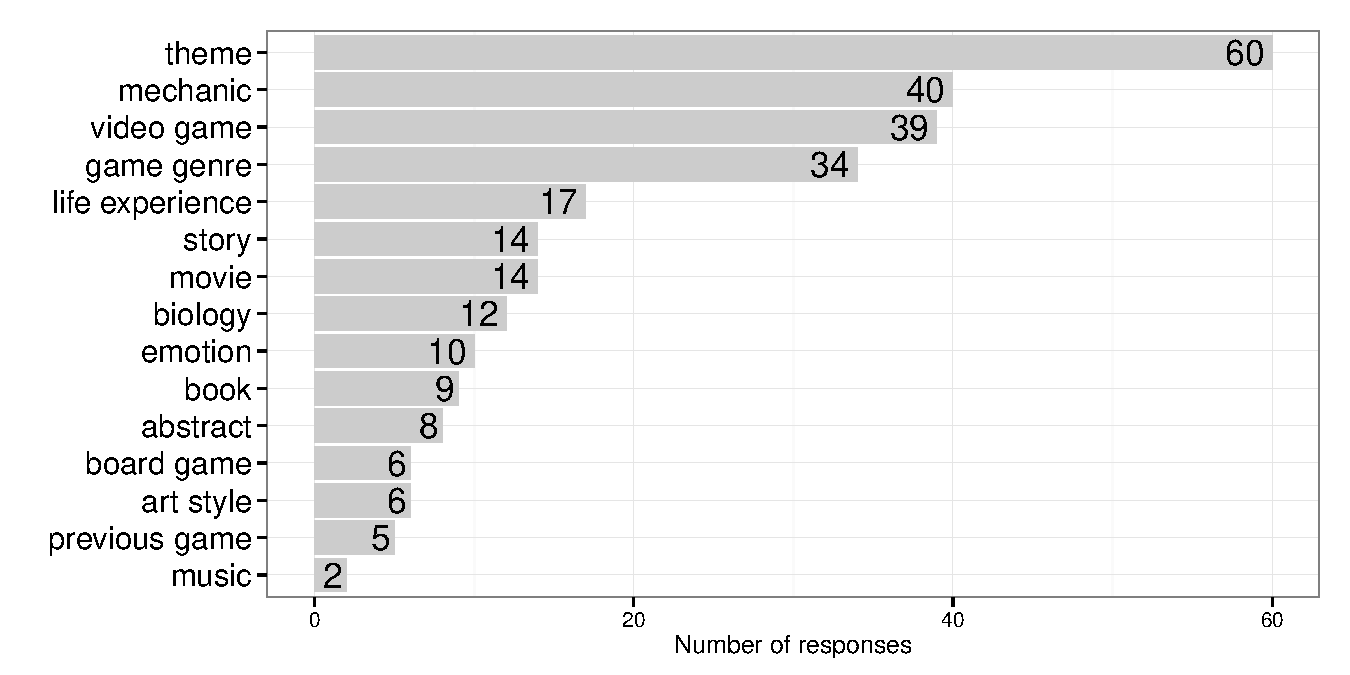
\includegraphics[width=0.7\linewidth]{./inspiration}
%}{%
%  \caption{A figure}%
%}
%\end{floatrow}
%\end{figure}

\begin{table}[tb]
\centering
\scriptsize
\begin{tabular}{|c|c|c|}
\hline coding & frequency & percentage \\ 
\hline theme & 60 & 21.7 \\ 
\hline mechanic & 40 & 14.5 \\ 
\hline other video game & 39 & 14.1  \\ 
\hline game genre & 34 & 12.3 \\ 
\hline life experience & 17 & 6.2 \\ 
\hline movie & 14 & 5.1 \\ 
\hline story & 14 & 5.1 \\ 
\hline biology & 12 & 4.3 \\ 
\hline emotion & 10 & 3.6 \\ 
\hline book & 9 & 3.3 \\ 
\hline abstract & 8 & 2.9 \\ 
\hline art style & 6 & 2.2 \\ 
\hline board game & 6 & 2.2 \\ 
\hline previously made game & 5 & 1.8 \\ 
\hline music & 2 & 0.7 \\ 
\hline 
\end{tabular}
\caption{Game inspiration sources.}
\label{tab:inspiration}
\end{table}

%Drawing from life experiences \cite{anthropy2012:zinesters}, systems to model \cite{crawford1984:gamedesign}, and other media \cite{bogost2011:howto} are all recognized in the game design literature as important sources of inspiration.
In general, the theme proved to be the most frequent starting point (60 out of 225 responses), followed by mechanics (40) and other games (39) or game genres (34).
%The heart beat theme lead many projects to emphasize rhythm mechanics or incorporate rhythm elements into another genre. 
Game references included specific digital games (e.g. Super Mario Bros.), playground or field games (e.g. Simon Says or tag), tabletop games (e.g. Hive), or game genres (e.g. platformer, card games). Other games inspired mechanics, art styles, controls, ``feel,'' and so on. 
Overall, game references targeted single-player games and action-oriented genres (side-scrolling runner, platformer, one-button games, etc.).

Life experiences used specific memories (e.g. watching a blind-friendly TV show) as well as general activities (e.g. holding a conversation).
Biological systems---particularly the heart and associated diseases---were a common source for system-oriented designs, primarily due to the heart beat jam theme.
Non-game media provided initial grounding through scenarios (e.g. Edgar Allan Poe's ``The Telltale Heart'') or more general characters and concepts (e.g. the Borg from ``Star Trek'').
Overall, these results show the breadth of topics addressed by GGJ participants is largely commensurate with industry and academic views, but scoped to meet the time demands of the GGJ \cite{bogost2011:howto}.

%Together, these results demonstrate the GGJ community matches many professional game design norms, skewed by the theme and limitations of the GGJ. The GGJ theme pushed many participants on more abstract concepts than often seen in industry staple titles focused on fantasy adventures and science fiction. Strict time and resource limits focused development on game genres that are quick and easy to implement and refine. 
%Together, these dual tensions make the GGJ a powerful incubator for small games that experiment with new themes and mechanics. However, this likely limits the value of the GGJ in training novices to build more complex game genres---real-time or turn-based strategy, role-playing games, simulation games, etc. Future GGJ efforts may target ways to support experimentation in these other avenues through alternative support structures, durations, or means for participating.

\subsection{Design Goals}
Three broad categories of goals drive GGJ participants: (1) personal goals, (2) player-oriented goals, and (3) system level goals.
Personal goals focused on benefits to GGJ participant themselves. 
The single most common goal (97 out of 288 answers) was to make and finish a game. 
Other personal goals included learning skills, networking with others, building a portfolio, test potential ideas for later expansion, enjoying the game creation process, or even ``win the competition.'' 
Participants see the jam as an opportunity to test out game development or seed their future projects.
An emphasis on competition among some is particularly interesting given the GGJ site explicitly states the GGJ is not a competition. %``The GGJ is not a competition.''\footnote{\url{http://globalgamejam.org/about}}

\begin{table}[tb]
\centering
\scriptsize
\begin{tabular}{|c|c|c|}
\hline coding & frequency & percentage \\ 
\hline make a game & 97 & 30.2 \\ 
\hline try out a mechanic & 48 & 15.0 \\ 
\hline have player enjoy & 44 & 13.7 \\ 
\hline learn skills & 33 & 10.3 \\ 
\hline recreate classic game & 25 & 7.8 \\ 
\hline convey a theme & 15 & 4.7 \\ 
\hline enjoy making a game & 15 & 4.7 \\ 
\hline be original & 13 & 4.0 \\ 
\hline meet people & 8 & 2.5 \\ 
\hline impact the player & 7 & 2.2 \\ 
\hline raise awareness of an issue & 6 & 1.9 \\ 
\hline test an idea & 4 & 1.2 \\ 
\hline win competition & 4 & 1.2 \\ 
\hline build portfolio & 2 & 0.6 \\ 
\hline 
\end{tabular} 
\caption{Goals for the game jam.}
\label{tab:goals}
\end{table}

Player-oriented goals emphasize the person(s) engaging with a game.
%Fullerton et al. \cite{fullerton2008:playcentric} emphasize a play-centric approach to design focusing on players while McGonigal \cite{mcgonigal2011:realitybroken} highlights the potential for games to have individual and societal impacts.
GGJ participants referenced goals of players enjoying the game, learning about a new topic (e.g. bee colony collapse disorder), or engaging in critical thinking about a topic. Societal-level design goals aimed to raise awareness about world issues or even ``change the world.''

System-level goals emphasized creating a game of a certain type (``old school point and click adventures'') or that meets certain design criteria (``multiplayer game with using [sic] physical mechanics''). Participants emphasized recreating other games, trying out new mechanics, having an original game, or attempting to convey a theme through the game structure. The GGJ theme and emphasis on innovation inspired some to set a goal for the final game system and strive to realize the conceived system in a concrete, running game.

Compared to the standard design mantra of focusing on player experience, the GGJ encourages a broader range of goals for personal gain, social improvement, or innovation. 


\subsection{Prototyping and Development Processes}
Relatively few respondents reported any form of prototyping (114 of 241 response). Many noted that their either was no time to prototype or that they considered their final game a prototype in itself. Others described a process that began as prototyping, but ended up being the final game.

\begin{table}[tb]
\centering
\scriptsize
\begin{tabular}{|c|c|c|}
\hline coding & frequency & percentage \\ 
\hline none & 127 & 52.7 \\ 
\hline game engine & 92 & 38.2 \\ 
\hline paper & 22 & 9.1 \\ 
\hline 
\end{tabular} 
\caption{Prototyping methods employed.}
\label{tab:prototyping}
\end{table}

\begin{table}[tb]
\centering
\scriptsize
\begin{tabular}{|c|c|c|}
\hline coding & frequency & percentage \\ 
\hline iterative & 67 & 72.0 \\ 
\hline quick & 26 & 28.0 \\ 
\hline 
\end{tabular} 
\caption{Prototyping processes followed.}
\label{tab:proto_process}
\end{table}

Prototyping processes broadly employed either paper prototyping (22) or engine prototyping (92).
Paper prototyping used whiteboards, paper drawings, or various tokens and pieces to simulate game systems and mechanics before beginning to code the game. Relatively few participants mentioned the use of paper prototypes, possibly due to lack of experience and familiarity or the limitations of the jam. Participants who did paper prototype described it as a beneficial practice:
``Complete paper prototype, make a turn-based version of the game. It was critical to nail the design in an hour and get working.''
%``[W]e used a simple paper prototype of poker chips on a grid to discuss and try various mechanics. It saved us a lot of programming time.''

Engine prototyping used game making software and engines (most commonly Unity) to test ideas or incrementally build up a core game. Mechanics, levels, characters, physics, controls, animations, movement, and user interfaces were all subject to this prototyping process. 
Participants often reported developing initial prototypes in game creation software intending to switch to a more complex development, only for the initial prototype to evolve into the final game. In these cases features were incrementally added to the initial game until the end of the jam.

Iterative development approaches (67 of 93) started from the core of the game before building upon it. Iterations would serially add new mechanics, add or improve art assets, or balance existing aspects of the game based on personal testing or outside playtest feedback.
Iterative development aimed to realize a pre-conceived game and hone its execution.
Unlike the case above, iterative development planned for the engine used to be the final game engine, rather than later switching implementation.

Test prototypes were used to explore potential ideas (26 of 93).
A quick baseline game would prove whether an idea was valuable or demonstrate a concept to others. Rarely (3 responses), this process would involve parallel creation of multiple ideas before selecting the design to use. 
Test prototypes sometimes became the final game, but conceptually differed from iterative prototyping. This approach used prototypes to test whether an idea was worth pursuing, rather than initiating the process of realizing a chosen idea.


\begin{table}[tb]
\centering
\scriptsize
\begin{tabular}{|c|c|c|}
\hline coding & frequency & percentage \\ 
\hline programming & 108 & 33.6 \\ 
\hline group members & 25 & 7.8 \\ 
\hline art & 25 & 7.8 \\ 
\hline time & 24 & 7.5 \\ 
\hline bugs & 20 & 6.2 \\ 
\hline none & 18 & 5.6 \\ 
\hline scoping & 18 & 5.6 \\ 
\hline source control / collaboration tools & 15 & 4.7 \\ 
\hline express idea in code & 16 & 5.0 \\ 
\hline balance & 16 & 5.0 \\ 
\hline planning and integration & 10 & 3.1 \\ 
\hline conceive idea & 10 & 3.1 \\ 
\hline ability to execute & 7 & 2.2 \\ 
\hline hardware & 5 & 1.6 \\ 
\hline audio & 4 & 1.2 \\
\hline 
\end{tabular}
\caption{Development problems.}
\label{tab:problem}
\end{table}

Development centered on learning tools to implement mechanics and removing game-breaking bugs. 
Respondents overwhelmingly indicated programming and acquiring and using game development tools as their most pressing challenges (107 of 280). 
Working with group members (25), meeting time constraints (24), making art (25), and fixing game bugs (20) were also important challenges. 
Scoping (17), game balance (12), converting concepts into code (14), and conceptualization (8) were lesser issues.
GGJ participants struggled to program their envisioned ideas, with design-level issues and asset creation as secondary concerns.

%Parallel development approaches built and tested features for the game in isolation before combining them into the final product. Many different systems were tested alone before combining them to yield a complete game. In contrast to serial approaches, these efforts focused on ensuring all the desired systems were functional before being combined by parallelizing work among team members.

%Compared to professionally described best practices \cite{fullerton2008:playcentric} 
%GGJ participants use relatively little player feedback. 

%Given the GGJ is focused on providing programming experience this may not necessarily be problematic, although future jams may consider alternative ways to prepare or support learning basic game creation tools before or during the jam to alleviate some of these problems.

\subsection{Game Evolution}
Realizing an initial game concept as an implemented game typically involved changing both the intended game features and in-game mechanics. 
%Responses to questions about changes to the game mechanics and game ideas were often interchangeable and we report on their combined results here.
GGJ participants managed the set of game features and game artifact in three ways:
(1) starting from many ideas and iteratively reducing scope;
(2) starting from vague ideas and building up mechanics and ideas through implementation;
and
(3) starting from a core idea and building it up based on testing and feedback.

\begin{table}[b]
\centering
\scriptsize
\begin{tabular}{|c|c|c|}
\hline coding & frequency & percentage \\ 
\hline none & 71 & 31.6 \\ 
\hline balance & 45 & 20.0 \\ 
\hline simplify & 27 & 12.0 \\ 
\hline scope & 24 & 10.7 \\ 
\hline add & 17 & 7.6 \\ 
\hline swap mechanics & 15 & 6.7  \\ 
\hline change visualization & 15 & 6.7 \\ 
\hline change controls & 7 & 3.1 \\ 
\hline fail to complete & 4 & 1.8 \\ 
\hline 
\end{tabular} 
\caption{Changes to design during the jam.}
\label{tab:sys_changes}
\end{table}

\begin{table}[tb]
\centering
\scriptsize
\begin{tabular}{|c|c|c|}
\hline coding & frequency & percentage \\ 
\hline feature cut & 59 & 21.2 \\ 
\hline none & 31 & 11.2 \\ 
\hline change details & 28 & 10.1 \\ 
\hline mechanic cut & 25 & 9.0 \\ 
\hline component cut & 24 & 8.6 \\ 
\hline mechanic swap & 20 & 7.2 \\ 
\hline feature add & 17 & 6.1 \\ 
\hline genre change & 17 & 6.1 \\ 
\hline visualization change & 13 & 4.7 \\ 
\hline story change & 12 & 4.3 \\ 
\hline idea change & 9 & 3.2 \\ 
\hline mechanic add & 9 & 3.2 \\ 
\hline visualization cut & 6 & 2.2 \\ 
\hline control change & 4 & 1.4 \\ 
\hline story cut & 4 & 1.4 \\ 
\hline 
\end{tabular} 
\caption{Changes to design ideas during jam.}
\label{tab:idea_changes}
\end{table}

Ideas were changed by: adding or removing planned mechanics, swapping out one mechanic for an (often simpler) alternative, and fine-tuning and balancing a mechanic. Some participants also included details on changes to the game objectives, story and theme, art assets and animations, or functionality of multiplayer interactions.

Scope reduction involved cutting planned features, reducing the complexity of mechanics or systems, or substituting complex mechanics with simpler alternatives (132 of 278).
Cutting features reduced the overall functionality of the game before implementation, typically because the magnitude of the task was unfeasible or time ran out. Participants removed systems within the game (e.g. attacks requiring combinations of buttons rather than single buttons) or reduced the total number of components used (e.g. fewer game levels or types of enemies).
Reducing mechanics occurred when already implemented systems were buggy or dysfunctional or when playtesting (personally or with others) showed them to be overly complex or unintuitive. 
Iterative scope reduction was the most common way participants described their process and was typically due to development constraints.

Concept development involved only vaguely specifying the game systems before building an initial game (38 of 278). Further mechanics and ideas were added to the game by expanding the core systems and crystallizing the general idea.
Rather than carefully plan out a full game, a vague inspiration would seed the process of solidifying ideas through incremental development: ``Mostly we talked the idea out, and just got to jamming. We iterated on the first prototype, and went from there.''
%``Come up with a game finishable in 4-8 hours and iterate from there.''
Extreme cases involved scrapping an initial idea and restarting (9) or changing the genre of a game after starting implementation (17). Concept development approaches emphasized exploring alternative ideas over detailed pre-planning.
%In some cases this lead to an unintentional change in game genre due to incremental shifts in mechanics or a shift in design goals:
%``Well because lack of fine tuning and testing, it turned out to be more time management game than rhythm-based on, which worked surprisingly well.''

Core idea expansion was a feedback-based approach that planned a small game and extended it through feedback (77 of 278). Changes to the game were typically additions to improve usability through better feedback to players or controls or changing out mechanics to better align with design goals. Unlike concept development, core idea expansion emphasized changing features based on testing feedback in order to refine and extend the game as needed. These approaches put heavier emphasis on a polished game design, rather than realizing a design concept idea.

Overall, GGJ participants tend to change game features, rather than compromise design ideas. Most development involved reducing the set of features implemented (132 of 278), refining initial ideas through feedback (77), or not changing the planned game at all (31). Openly exploring possible designs was comparatively rare (38). Features are more likely to change than the design ideas. Together, these results paint a picture of GGJ development as focused on delivering a planned idea, rather than experimenting with possible ideas.

\section{Methodological Implications}
% % note limitations of survey method: wasn't able to get great detail on flow of process; focus on high-level changes; only those who opt-in
Our voluntary survey methodology has important limitations in coverage of GGJ participants and the depth of response data gathered. Only 419 of 16,705 participants responded to these questions. Respondents were likely skewed toward successful projects and those more invested in the GGJ. Thus, we cannot easily examine similarities or differences in design processes between those who successfully complete the GGJ and those who do not. Future research will require better methods to automate survey administration and collection or ensure randomized sampling from participants.

Survey responses are limited to the most salient aspects of an experience, limiting the level of detailed processual information gathered. We cannot make strong conclusions about the cognitive or social processes involved in game development from this form of data. Retrospective protocol analysis---where participants are recorded and asked to then view this recording and narrate their thinking---is one means to gather such detailed data, although constrained to a smaller scale than we studied. Retrospective protocols are typically used for short sessions (up to hours). Modifications for longer duration events may review only key points in the process or to use a ``fast-forward'' viewing approach. 

Semi-structured interviews support a more exploratory approach to collecting detailed data. Interviews are limited by being subjective data, but require far less time and detailed data than protocol analysis while still gaining useful qualitative insights. Using prompt materials gathered over the course of the GGJ---such as in-process game builds from source control, photos or video of onsite activity, and observer notes on the development process---may ameliorate participant biases around memory salience.

Our survey did not have identifying information on participants. Thus, we could not study of how collaboration impacts the conceptualization and development process at the GGJ. Employing a retrospective protocol or semi-structured interview with individuals and then groups is one means to collect such information.


\section{Discussion}
To date, game design processes have been examined using personal reflection \cite{anthropy2012:zinesters,hunicke2004:mda}, small-scale individual interaction \cite{nelson2009:reqanal}, or study of complete games \cite{bogost2011:howto}. We complement this work by providing a large-scale analysis of time-constrained game design, illustrating trends in development processes. 
GGJ participants and use diverse inspirations and set goals for their personal benefit, the impact on game players, and structure of the game system.
Participants rarely employ traditional prototyping, instead evolving their games by scoping down many ideas, concretizing a vague idea through implementation, and iteratively expanding a simple core game.

Our results indicate rich potential for more fine-grained analysis to uncover the relationships between processes and development outcomes. Designers vary in scoping, concretizing, or expanding out initial ideas. Our preliminary study opens a number of future research questions. How do final products of these methods differ? Which aspects of games are amenable to incremental addition and which must be present from the start? How do designers recognize dependencies among game systems and prioritize them? Relating design processes to outcomes is crucial for better structuring future jams, game development instruction, and tools.

Many designers struggled to implement their envisioned game systems and mechanics. How do they go about realizing the mapping of a mechanic concept to pieces of running code? Further, development was typically iterative. What kinds of feedback do designers use to guide development? How is feedback interpreted? What guides decisions to cut features as opposed to adjust the game engine? Understanding the feedback loop between a running game and design concepts can inform methods for teaching designers and building better game development technologies.

Investigating the questions above poses methodological challenges for collecting and annotating data at a sufficient scale. Surveys provide useful qualitative results to develop theory, but require more in-depth qualitative methods to uncover deeper process-level details. Automated recording of game development processes and annotating these records are one means to enable quantitative analysis at the massive scale the GGJ provides. 
Future research should build on these results to examine fine-grained details of time-constrained game development and develop new methodologies to leverage the potential of massive development information from sources like the GGJ.

%ACKNOWLEDGMENTS are optional
%\section{Acknowledgments}
%Global Game Jam committee. Global Game Jam participants and survey respondents.


% The following two commands are all you need in the
% initial runs of your .tex file to
% produce the bibliography for the citations in your paper.
\bibliographystyle{abbrv}
\bibliography{lib}


% ACM needs 'a single self-contained file'!

%\pagebreak

%APPENDICES are optional
%\balancecolumns
\appendix
%\todo[inline]{possibly use for questions given}
\section{Survey Questions}
\label{sec:survey}
\begin{list}{\labelitemi}{\leftmargin=10pt \itemindent=0em \itemsep=0pt}
\item What was your initial goal for the game you made during the global game jam?
\item What inspirations or initial ideas did you have for your game? What was the starting inspirational source or goal for the game?
\item Why did you pick this particular idea for the game?
\item What problems did you encounter in developing your game?
\item What changes did you make to your initial idea as you worked on it during the game jam? Please describe the changes as small pieces of changes as possible.
\item What game mechanics and/or gameplay systems did you use in your game?
\item How did the mechanics or systems you made relate to the initial design ideas you had?
\item How did these mechanics change as you worked on the game during the game jam?
\item Did you prototype your game? If so, what kind of prototyping did you do and what did you learn from doing it?
%\item What tools did you use to make your game? Please include software tools (e.g. programming languages or game engines) and any physical/analog materials (e.g. paper prototyping methods or storyboarding).
\end{list}


%\begin{table}
%\begin{tabular}{|p{\linewidth}|}
%\hline What was your initial goal for the game you made during the global game jam? \\
%\hline What inspirations or initial ideas did you have for your game? What was the starting inspirational source or goal for the game? \\
%\hline Why did you pick this particular idea for the game? \\
%\hline What problems did you encounter in developing your game? \\
%\hline What changes did you make to your initial idea as you worked on it during the game jam? Please describe the changes as small pieces of changes as possible. \\
%\hline What game mechanics and/or gameplay systems did you use in your game? \\
%\hline How did the mechanics or systems you made relate to the initial design ideas you had? \\
%\hline How did these mechanics change as you worked on the game during the game jam? \\
%\hline Did you prototype your game? If so, what kind of prototyping did you do and what did you learn from doing it? \\
%\hline What tools did you use to make your game? Please include software tools (e.g. programming languages or game engines) and any physical/analog materials (e.g. paper prototyping methods or storyboarding). \\
%\hline 
%\end{tabular}
%\caption{Survey questions.}
%\label{tab:survey} 
%\end{table}

\end{document}
